\section{Introduction}\label{sec:intro}
As the field of wireless sensor networks has grown the past years, so too has the range of applications proposed for this technology. This diversity translates to differing requirements from the underlying sensor network. Many different models and protocols has been proposed for the different layers of the
network stack have been designed \cite{WSNpaper}. Strategies that allow for energy saving, lower computations  and overhead, distance estimation and location of nodes, link quality estimations, authentication to achieve security requirements and many other parameters relevant to their performance.
\\[8pt]
This paper is based upon the ideas presented by Dong et al. in their study of packet length optimization schemes \cite{DPLCpaper}. They present a lightweight dynamic packet length scheme based on a link estimation method designed to capture both physical channel conditions and interference. Further, they demonstrate the effectiveness of the scheme on a testbed of TelosB motes. The purpose of the scheme is to adjust the payload size of messages, which is a change that is readily made dynamically, since it requires little extra effort from the sensors, as opposed to dynamically adjusting other factors such as bit rate or implementing coding schemes. The reasoning behind adjusting the payload size is the fact that as packets grow larger, it is more likely that a part of the packet becomes corrupted, thus causing the packet to be dropped at the receiver. However, since the packet header has a fixed size the overhead will be larger for small packets, reducing the effective throughput. As an example, in case of TelosB motes, the radio chip CC2420 uses the IEEE 802.15.4 protocol, where the PHY+MAC headers are at least 11 bytes, depending on the adressing information contained \cite{CC2420}.
\\[8pt]
The paper is organized as follows: In section \ref{sec:pacSizeInf}, the influence of changing the packet length is investigated, by calculation the analytical result in a Binary Symmetric Channel (BSC). Section \ref{sec:chanEst} takes this into the real world, showing measurements of what the effect really is. Then, section \ref{sec:DPLC} presents a simple scheme that allows a sensor mote to dynamically adjust the payload size to continously maximize transmission efficiency. This effectiveness of this scheme is then shown, first in section \ref{sec:simScheme}, with simulation under the BSC assumption, and then in section \ref{sec:schemeTest}, where a real implementation of the scheme is demonstrated. Finally, the paper ends with a presentation of further work and a conclusion in sections \ref{sec:FW} and \ref{sec:conclusion}.
\\[8pt]
The main contribution of this paper is an investigation of the possibility of changing packet length to maximize transmission efficiency, as well as presentation and evaluation of a simple scheme that is able to do this.
\section{Packet Size Influence}\label{sec:pacSizeInf}
In order to understand the effects of adjusting the packet length, an analytical result is presented. First, the transmission efficiency $\mathcal{E}$, which is the amount of useful information bits received per transmitted bit, is:
\begin{equation}
\mathcal{E}(l) = \frac{l\cdot \text{p}(l)}{l + H + O},\label{E}
\end{equation}
where $l$ is the payload length, $p(l)$ is the packet reception rate (PRR) when packets have length $l$, $H$ is overhead from the header and $O$ is additional overhead introduced by the optimization scheme \cite{DPLCpaper}. Since the scheme is not yet considered, let $O=0$ for now. Under the assumption that the channel is a Binary Symmetric Channel (BSC), the analytical value of $\mathcal{E}$ can be found. Assuming that the receiver is able to correctly detect whenever the message is incorrectly received, and has no correction capability, a packet will be passed to the higher layers only when no changes to it were introduced by the channel. The packet reception rate is then:
\begin{equation}
p(l) = (1 - p)^{l+H},
\end{equation}
where $p$ is the probability of a bit flipping in the channel. This can be used to calculate the theoretical efficiency, based on equation (\ref{E}). The result for $p=0.01$ is shown on figure \ref{fig:BSC}, with $l\in \{11,12,...,127\}$, the frame sizes possible with 802.15.4 \cite{CC2420}. It is clearly seen that there is a best efficiency $\mathcal{E}_{opt} = 0.49$ at $l_{opt} = 39$ for this specific channel. It is seen that the PRR is decreasing sharply as packet size increases. In reality, the assumption of a BSC might actually be too strict, since the BSC has an equal chance of introducing an error on any bit, whereas a burst error channel could suffer fading in an interval, causing many errors in one packet, but still only causing one packet to be dropped. This is a more difficult channel model to analyze, but it is still reasonable to conclude that longer packets will be more likely to be dropped, as the entire packet should likely be received whenever the channel is in a good state, unless the state changes during transmission.
\begin{figure}
\centering
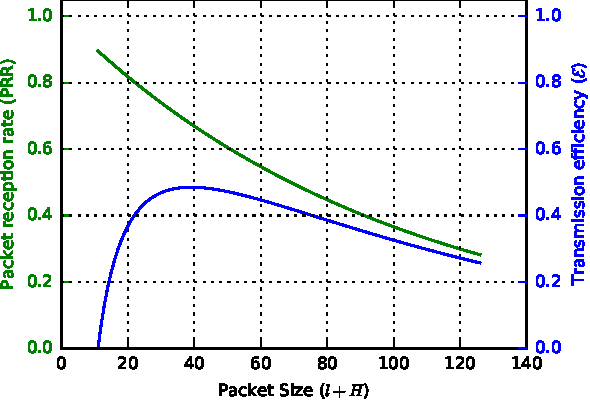
\includegraphics[scale=1]{figs/simFig_BSC001.pdf} 
\caption{\textit{Packet reception rate and Transmission efficiency for BSC with $p=0.01$.}\label{fig:BSC}}
\end{figure}